%--- 1 ----------------------------------------------------------
\item\qouv{Définissez ce qu’est un design pattern, comment le caractériser et à quoi il sert.}
{Un design pattern est un \textbf{modèle de conception} général qui répond à une problématique récurrente en développement. Il s'agit d'une desciption de solution dont l'implémentation doit être adpatée aux cas particulier.
\paragraph{}
Les patterns sont donc utilisés pour simplifier la vie des programmeurs, ils représentent un gain de temps (ne pas réinventer la roue) et une fiabilité puisqu'ils s'agit de modèles testés et approuvés avec le temps.

\paragraph{}
Un pattern est définit par:
\begin{itemize}
\item[$\cdot$]un \textbf{nom}
\item[$\cdot$]une \textbf{description du problème} auquel il s'applique
\item[$\cdot$]la \textbf{solution}: générique!! Son implémentation est à adapter au cas par cas
\item[$\cdot$]les \textbf{conséquences} de son utilisation: peut avoir des répercutions sur le reste du code, forcer des choix d'implémentation allieurs,...
\end{itemize}

\paragraph{}
Il existe 23 patterns \textit{classiques}, définis par le GoF, regroupés selon trois catégories:
\begin{enumerate}
\item \textbf{construction}: concerne l'instanciation des classes
\item \textbf{structuraux}: concerne l'organisation des classes entre elles
\item \textbf{comportementaux}: concerne la communication entre les objets
\end{enumerate}
}

%--- 2 ----------------------------------------------------------
\item\qouv{Que sont les concurrency patterns ? Donnez quelques exemples.}
{Ce sont des patterns utilisés pour de la \textbf{programmation concurrente}.
Ils apportent entre autre des modèles pour: la synchronisation, la communication, le stockage de données, les caches,...\paragraph{EXEMPLES [...]}
}

%--- 3 ----------------------------------------------------------
\item\qouv{Décrire ce qu’est le test driven development (TDD).}
{Le cycle TDD définit une méthode de développement qui consiste à être \textbf{guidé par l'écriture de tests} et intégrer des phases de refactoring.
\paragraph{}
La figure ci-dessous définit les trois grandes étapes de chaque tour de cycle. La deuxième étape consiste à écrire un code permettant de passer le(s) test(s) -> on ne parle encore d'optimisation. C'est seulement à l'étape 3, lorsque le code est fonctionnel, que l'on peut penser à des améliorations pour éliminer les \textit{bad smells}.
\begin{figure}[h!]
\center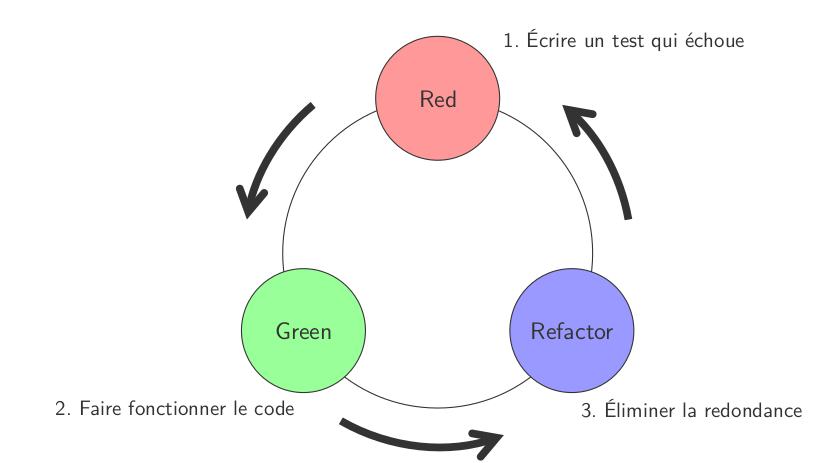
\includegraphics[scale=.4]{images/cycle-tdd}
\caption{Le cycle TDD selon Kent Beck}
\end{figure}

}

%--- 4 ----------------------------------------------------------
\item\qouv{Définissez ce qu’est un bad smell et donnez un exemple.}
{Un \textit{bad smell} est une \textbf{faiblesse de codage} dans un programme, il ne s'agit pas d'un bug!!!
\paragraph{}Exemples de bad smells:
\begin{itemize}\setlength{\itemsep}{.3em}
\item[$\cdot$] \textbf{Large class (the blob)}: une classe (God class) monopolise tout le traitement et les autres stockent uniquement des données -> va à l'encontre du principe de POO "une classe = une responsabilité". La \textit{God Class} utilise des détails d'implémentation des autres classes -> va à l'encontre de l'encapsulation.
\item[$\cdot$]\textbf{code dupliqué}: du code identique ou très similaire à différents endroits dans le programme -> difficile à maintenir. Il faut isoler les parties communes dans des métodes.
\item[$\cdot$]\textbf{Long method}: méthode dont le coprs possède beaucoup d'instructions -> limite la réutilisabilité et difficile à comprendre. Une méthode ne devrait avoir qu'une seule fonctionnalité.
\item[$\cdot$]...
\end{itemize}
}

%--- 5 ----------------------------------------------------------
\item\qouv{Définissez ce qu’est le refactoring et à quel moment il peut être utilisé dans le processus de
développement.}
{Le refactoring consiste à transformer du code tout en \textbf{préservant son comportement}, il s'agit donc d'\textbf{améliorer la qualité} d'un code déjà fonctionnel.
\paragraph{}
Cette technique s'inscrit dans la logique d'\textit{optimisation du code}, dont un principe fondamental est le suivant: \textit{"l'optimisation ne doit intervenir qu'une fois que le programme fonctionne et répond aux spécifications fonctionnelles."}
\paragraph{}
Dans le cas d'un cycle TDD (Test-Driven Development, voir Q3), le réfactoring du code a donc lieu après que celui-ci ait passé une batterie de tests. L'idée est de se servir de ces mêmes tests pour s'assurer que les modifications n'aient pas altéré le bon fonctionnement du code.

\paragraph{EXEMPLES [...]}

\paragraph{Remarque: }
l'étape de refactoring n'ajoute pas de fonctionnalité et ne corrige pas de bug !! On re-travaille un code dans le but d'améliorer sa lisibilité et sa maintenance mais son comportement externe reste identique.

}

%--- 6 ----------------------------------------------------------
\item\qouv{Définissez la notion de paradigme de programmation, ainsi que la programmation impérative et
déclarative.}
{}

%--- 7 ----------------------------------------------------------
\item\qouv{Définissez la notion de système distribué en reprenant rapidement les cinq buts.}
{}

%--- 8 ----------------------------------------------------------
\item\qouv{Définissez la notion de middleware. Dans quel type d’architecture les retrouve-t-on ?}
{}

%--- 9 ----------------------------------------------------------
\item\qouv{Donnez la différence entre un client léger et lourd, dans une architecture client-serveur.}
{}

%--- 10 ----------------------------------------------------------
\item\qouv{Qu’est-ce-que CORBA et quel type d’architecture supporte-t-il ?}
{}